\documentclass[11pt,a4paper]{article}
\usepackage[utf8]{inputenc}
\usepackage[T1]{fontenc}
\usepackage[sc]{mathpazo}
\usepackage[scaled=0.92]{helvet}
\usepackage{microtype}
\usepackage[a4paper,top=2.6cm,bottom=2.4cm,left=2.4cm,right=2.4cm,headheight=14pt]{geometry}
\usepackage[table]{xcolor}
\usepackage{booktabs,array,enumitem,multirow}
\usepackage{tikz}
\usetikzlibrary{calc,positioning}
\usepackage{pgfplots}
\pgfplotsset{compat=1.16}
\usepackage[most]{tcolorbox}
\usepackage{titlesec}
\usepackage{needspace,etoolbox}
\usepackage{fancyhdr}
\usepackage{caption}
\usepackage{url}
\def\UrlBreaks{\do\/\do\-\do\_\do\.\do\=\do\?\do\&\do\a\do\b\do\c\do\d\do\e\do\f\do\g\do\h\do\i\do\j\do\k\do\l\do\m\do\n\do\o\do\p\do\q\do\r\do\s\do\t\do\u\do\v\do\w\do\x\do\y\do\z}
\Urlmuskip=0mu plus 1mu
\urlstyle{same}
\usepackage[hidelinks]{hyperref}

% ---- Palet (selaras dengan halaman dokumen pelengkap) ----
\definecolor{teal}{HTML}{0A6C6E}
\definecolor{tealdark}{HTML}{07484A}
\definecolor{ink}{HTML}{13262A}
\definecolor{muted}{HTML}{51666A}
\definecolor{rule}{HTML}{D3DEDC}
\definecolor{pale}{HTML}{EEF5F4}
\definecolor{amber}{HTML}{B7791F}
\definecolor{amberpale}{HTML}{FBF4E4}
\definecolor{well}{HTML}{CFE3E0}

\renewcommand{\tablename}{Tabel}
\renewcommand{\figurename}{Gambar}
\renewcommand{\refname}{Daftar Pustaka}
\color{ink}
\setlength{\parindent}{0pt}
\setlength{\parskip}{6.5pt plus 1pt}
\linespread{1.06}
\tolerance=1200
\emergencystretch=3em
\hyphenpenalty=1500
\setlist{itemsep=2.5pt,topsep=3pt,parsep=0pt,leftmargin=1.4em}
\setlist[itemize]{label={\color{teal}\textbullet}}
\renewcommand{\arraystretch}{1.22}
\setlength{\tabcolsep}{5pt}
\captionsetup{font={small,sf,color=muted},labelfont={bf,color=teal},labelsep=period,justification=raggedright,singlelinecheck=false,skip=5pt}

% ---- Judul bagian ----
\titleformat{\section}{\sffamily\bfseries\Large\color{ink}}{\color{teal}\thesection}{0.7em}{}[{\color{rule}\titlerule[0.6pt]}]
\titlespacing*{\section}{0pt}{18pt}{9pt}
\titleformat{\subsection}{\sffamily\bfseries\normalsize\color{tealdark}}{\color{teal}\thesubsection}{0.6em}{}
\titlespacing*{\subsection}{0pt}{11pt}{3pt}

% ---- Kepala dan kaki halaman ----
\pagestyle{fancy}
\fancyhf{}
\renewcommand{\headrulewidth}{0pt}
\fancyhead[L]{\sffamily\scriptsize\color{muted}\textsc{Alergen}\ \raisebox{0.15ex}{\tiny$\bullet$}\ Studi Kelayakan Skala Nasional}
\fancyhead[R]{\sffamily\scriptsize\color{muted}Kit Diagnostik Alergi Berbasis Patch}
\fancyfoot[L]{\sffamily\scriptsize\color{muted}Universitas Airlangga \ $\cdot$ \ IDS000011522}
\fancyfoot[R]{\sffamily\small\bfseries\color{teal}\thepage}
\renewcommand{\headrule}{\color{rule}\hrule width\headwidth height 0.5pt}
\renewcommand{\headrulewidth}{0.5pt}
\fancypagestyle{plain}{\fancyhf{}\renewcommand{\headrulewidth}{0pt}\fancyfoot[R]{\sffamily\small\bfseries\color{teal}\thepage}}

% ---- Tabel ----
\newcommand{\tH}[1]{\textcolor{white}{\sffamily\bfseries\small #1}}
\newcommand{\tabstart}{\small\rowcolors{2}{white}{pale}\arrayrulecolor{rule}}
\newcommand{\hdrrow}{\rowcolor{tealdark}}
\newcolumntype{L}[1]{>{\raggedright\arraybackslash}p{#1}}
\newcolumntype{R}[1]{>{\raggedleft\arraybackslash}p{#1}}
\setlength{\aboverulesep}{0pt}\setlength{\belowrulesep}{0pt}
\renewcommand{\toprule}{\arrayrulecolor{tealdark}\specialrule{0.9pt}{0pt}{0pt}\arrayrulecolor{rule}}
\renewcommand{\bottomrule}{\arrayrulecolor{tealdark}\specialrule{0.9pt}{0pt}{0pt}\arrayrulecolor{rule}}

% ---- Kotak catatan dan kartu angka ----
\newtcolorbox{catatan}[1][Catatan]{enhanced,breakable,colback=amberpale,colframe=amberpale,boxrule=0pt,
  borderline west={2.2pt}{0pt}{amber},arc=1.5pt,left=10pt,right=8pt,top=6pt,bottom=6pt,
  before skip=8pt,after skip=10pt,
  title={\sffamily\bfseries\small\color{amber}\MakeUppercase{#1}},coltitle=amber,
  attach boxed title to top left={yshift=-2mm,xshift=0pt},boxed title style={empty,left=0pt,top=0pt,bottom=0pt},
  fonttitle=\sffamily,coltext=ink,before upper={\vspace{2pt}}}
\newtcolorbox{kartu}[2]{enhanced,colback=pale,colframe=pale,boxrule=0pt,arc=3pt,
  left=8pt,right=6pt,top=6pt,bottom=6pt,halign=left,
  borderline west={2.5pt}{0pt}{teal},
  before upper={{\sffamily\bfseries\LARGE\color{teal}#1}\par\vspace{1pt}},
  fontupper=\sffamily\scriptsize\color{muted},height=1.95cm,valign=top}
\newcommand{\kartuRow}[4]{%
 \begin{tcbraster}[raster columns=#1,raster equal height,raster column skip=7pt,raster row skip=7pt]#2#3#4\end{tcbraster}\vspace{9pt}}

% ---- Sampul ----
\newcommand{\patchmotif}[2]{% #1 skala, #2 warna garis
 \begin{scope}[scale=#1]
 \draw[#2,line width=1.2pt,rounded corners=9pt] (0,0) rectangle (15,6);
 \foreach \r in {0,1}{\foreach \c in {0,...,4}{
   \draw[#2,line width=1pt] ({1.9+\c*2.7},{4.1-\r*2.2}) circle (0.9);}}
 \end{scope}}

\newcommand{\makecover}[5]{% kode, judul, subjudul, tagline, ringkasan satu kalimat
\begin{titlepage}
\thispagestyle{empty}
\begin{tikzpicture}[remember picture,overlay]
 \fill[tealdark] (current page.north west) rectangle ($(current page.north east)+(0,-17.2cm)$);
 \fill[teal!85!tealdark] ($(current page.north east)+(0,-17.2cm)$) -- ($(current page.north east)+(-10cm,-17.2cm)$) -- ($(current page.north east)+(0,-10.8cm)$) -- cycle;
 \begin{scope}[shift={($(current page.north east)+(-9.9cm,-6.4cm)$)}]
   \patchmotif{0.5}{white!35}
 \end{scope}
 \node[anchor=north west,text=white!70,font=\sffamily\small\bfseries,align=left] at ($(current page.north west)+(2.4cm,-2.7cm)$) {\textsc{Alergen \ $\cdot$ \ Universitas Airlangga}};
 \node[anchor=north west,text=white,font=\sffamily\bfseries\fontsize{44}{44}\selectfont] at ($(current page.north west)+(2.4cm,-7.4cm)$) {#1};
 \node[anchor=north west,text=white,font=\sffamily\bfseries\fontsize{26}{31}\selectfont,text width=14.2cm,align=left] at ($(current page.north west)+(2.4cm,-10.2cm)$) {#2};
 \node[anchor=north west,text=white!85,font=\sffamily\fontsize{13}{17}\selectfont,text width=14cm,align=left] at ($(current page.north west)+(2.4cm,-14.1cm)$) {\hyphenpenalty=10000\exhyphenpenalty=10000 #3};
 \node[anchor=north west,text=ink,font=\fontsize{12}{17}\selectfont,text width=15.2cm,align=left] at ($(current page.north west)+(2.4cm,-18.8cm)$) {#4};
 \draw[teal,line width=2pt] ($(current page.north west)+(2.4cm,-21.9cm)$) -- ++(2.2cm,0);
 \node[anchor=north west,text=muted,font=\sffamily\small,text width=15cm,align=left] at ($(current page.north west)+(2.4cm,-22.4cm)$) {%
  \textbf{\color{ink}Kit Diagnostik Alergi Berbasis Patch (Alergen)}\\[3pt]
  Universitas Airlangga, Surabaya\\
  Paten Sederhana IDS000011522\\
  Oktober 2026};
 \node[anchor=south east,text=muted,font=\sffamily\scriptsize,align=right] at ($(current page.south east)+(-2.4cm,1.6cm)$) {#5};
\end{tikzpicture}
\end{titlepage}
\newpage}

\definecolor{sr1}{HTML}{8AA6AB}
\definecolor{sr2}{HTML}{3FA7A3}
\definecolor{sr3}{HTML}{0A6C6E}
\definecolor{sr4}{HTML}{B7791F}
\pgfplotsset{natbase/.style={width=0.95\linewidth,height=6.2cm,
  every axis label/.append style={font=\sffamily\scriptsize,color=muted},
  tick label style={font=\sffamily\scriptsize,color=muted},
  legend style={font=\sffamily\scriptsize,draw=rule,fill=white,at={(0.5,-0.2)},anchor=north},
  grid=major,grid style={color=rule,line width=0.4pt},
  axis line style={color=rule},tick style={color=rule},
  scaled ticks=false,/pgf/number format/.cd,1000 sep={.},fixed,precision=0,/tikz/.cd},
  natplot/.style={natbase,xtick={1,2,3,4,5},xticklabels={2028,2029,2030,2031,2032}}}
\hypersetup{pdftitle={Studi Kelayakan Skala Nasional},pdfauthor={Tim Alergen, Universitas Airlangga}}

\pretocmd{\section}{\Needspace{7\baselineskip}}{}{}
\pretocmd{\subsection}{\Needspace{4\baselineskip}}{}{}


\begin{document}

\makecover{Kelayakan}{Studi Kelayakan Skala Nasional}{Peluncuran bertahap kit diagnostik alergi berbasis patch di seluruh Indonesia}{Dokumen ini menilai kelayakan komersial kit pada skala nasional: pasar, strategi peluncuran, kebutuhan produksi, keuangan, kekayaan intelektual, dan risiko. Angka dasar, asumsi tambahan, dan angka dari sumber luar dipisahkan agar mudah diperiksa.}{Seluruh angka dihitung dengan skrip yang dapat dijalankan ulang}

\section*{Ringkasan}
\addcontentsline{toc}{section}{Ringkasan}

\kartuRow{4}
{\begin{kartu}{3.334}{}kit per tahun: titik impas pada biaya tetap Rp300 juta\end{kartu}}
{\begin{kartu}{1.338}{}fasilitas aktif pada 2032, skenario nasional dasar\end{kartu}}
{\begin{kartu}{Rp20,07}{}miliar rupiah: omzet 2032, skenario nasional dasar\end{kartu}
\begin{kartu}{5,8 tahun}{}sisa masa paten, berakhir 11 Agustus 2032\end{kartu}}

Dokumen ini menilai apakah kit dapat dijual secara nasional, bukan hanya di beberapa fasilitas. Kit masih berupa prototipe tanpa validasi pada manusia dan tanpa izin edar, sehingga seluruh angka di bawah adalah \textbf{skenario}, bukan prakiraan penjualan.

\begin{itemize}
\item \textbf{Pasar.} Indonesia berpenduduk 284,67 juta jiwa. BPJS Kesehatan bekerja sama dengan 26.759 fasilitas kesehatan, dan peserta JKN mencapai 282,7 juta jiwa, lebih dari 98\% penduduk. Pulau Jawa dihuni 56,10\% penduduk.
\item \textbf{Harga per alergen.} Kit memuat 10 alergen, atau Rp15.000 per alergen pada harga neto. Dibanding panel IgE 54 alergen di RS Royal Progress (Rp40.741 per alergen), harga kit 37\%, atau 74\% dengan margin fasilitas 100\%. Harga panel kecil 10 sampai 20 alergen jauh lebih tinggi per alergen, sehingga setara 10 alergen berkisar Rp725.000 sampai Rp1.164.500. Model memakai dua pembanding, yaitu Rp407.407 (konservatif) dan Rp1.000.000 (panel kecil).
\item \textbf{Skenario.} Empat skenario lima tahun dibandingkan: regional (200 fasilitas pada 2032) dan tiga skenario nasional dengan adopsi 2\%, 5\%, dan 10\% dari seluruh fasilitas mitra BPJS pada 2032. Pada skenario nasional dasar, kit dipakai di 1.338 fasilitas dan terjual 133.800 kit pada tahun ke-5, setara 47,0 pemeriksaan per 100.000 penduduk.
\item \textbf{Titik impas.} Pada biaya tetap dasar Rp300 juta, titik impas hanya 34 fasilitas. Bila biaya tetap skala nasional 10 kali lebih besar (Rp3,0 miliar per tahun, asumsi sensitivitas), titik impas menjadi 33.334 kit atau 334 fasilitas (1,2\% dari seluruh fasilitas mitra).
\item \textbf{Investasi.} Investasi awal belum tersedia. Pada skenario nasional dasar, investasi yang masih menghasilkan NPV nol pada diskonto 20\% adalah Rp10,7 miliar (biaya tetap dasar) atau Rp2,6 miliar (biaya tetap Rp3,0 miliar). Skenario regional tidak menopang investasi sebesar itu pada biaya tetap yang lebih tinggi.
\item \textbf{Paten.} Masa paten berakhir 11 Agustus 2032 dan tidak dapat diperpanjang. Royalti dari paten ini saja bernilai Rp290 juta sampai Rp876 juta pada skenario nasional dasar. Nilai jangka panjang ada pada volume, know-how, dan lapisan KI tambahan.
\item \textbf{Syarat penentu.} Kepastian klasifikasi dan jalur izin edar, bukti validasi klinis, standardisasi ekstrak alergen, kapasitas produksi sekitar 11.150 kit per bulan pada tahun ke-5, dan perjanjian yang mengikat dengan mitra produksi dan distribusi.
\end{itemize}

\begin{catatan}[Cara membaca angka]
Skenario nasional memakai harga neto, biaya variabel, dan 100 kit per fasilitas per tahun sebagai asumsi dasar. Jumlah fasilitas aktif, biaya tetap skala nasional, dan jadwal peluncuran adalah asumsi tambahan yang dapat diubah di skrip model.
\end{catatan}

\section{Produk dan posisinya}

Produk berupa patch berukuran 2 $\times$ 5 cm dengan sumur berdiameter 7 mm untuk sepuluh ekstrak alergen: tungau debu, udang, susu sapi, daging, ayam, telur, gandum, kacang tanah, kelapa, dan polen. Polimer membawa ekstrak, dan seal pelindung menutup bagian patch sebelum dipakai. Reaksi kulit dibaca dengan aplikasi seluler yang memberi skor dari foto patch. Status saat ini adalah prototipe. Landasan awal berupa studi in vitro pematangan sel dendritik (penanda CD209 dan CD86), sedangkan keamanan, kinerja diagnostik, waktu baca, dan kriteria interpretasi pada manusia masih harus divalidasi.

Tabel~\ref{tab:pos} menempatkan produk di antara pendekatan yang sudah ada. Cakupannya sepuluh alergen, jauh lebih sempit daripada panel IgE spesifik 54 sampai 96 alergen \cite{royal,pramita}. Pembanding patch yang paling dekat adalah T.R.U.E. TEST, yang berlisensi biologik di Amerika Serikat untuk membantu diagnosis dermatitis kontak alergi, bukan untuk alergi makanan atau inhalan \cite{fda}.

\begin{table}[htbp]
\centering
\caption{Posisi produk terhadap pendekatan pemeriksaan alergi.}
\label{tab:pos}
\tabstart
\begin{tabular}{@{}L{3.0cm}L{5.0cm}L{6.9cm}@{}}
\toprule
\hdrrow\tH{Pendekatan} & \tH{Prinsip} & \tH{Catatan untuk posisi produk} \\
\midrule
Uji tusuk kulit & Alergen masuk melalui tusukan kulit & Metode in vivo yang paling umum pada laporan pasar \cite{gmi}; produk berfokus pada aplikasi tanpa penusukan \\
IgE spesifik (darah) & Sampel darah dan fasilitas laboratorium & Termasuk segmen in vitro \cite{gmi}; produk tidak memerlukan laboratorium untuk aplikasi \\
Patch dermatitis kontak & Evaluasi reaksi tipe lambat; contoh T.R.U.E. TEST dengan 35 alergen pada tiga panel & Indikasi dermatitis kontak alergi usia 6 tahun ke atas \cite{fda}; bukan pembanding untuk alergen makanan dan inhalan \\
Patch Alergen (produk ini) & Sepuluh ekstrak alergen makanan dan inhalan pada satu patch dengan pembacaan aplikasi & Kinerja diagnostik dan kriteria interpretasi belum divalidasi pada manusia \\
\bottomrule
\end{tabular}
\end{table}

\section{Pasar nasional}

\subsection{Pasar global sebagai arah}

Laporan riset pasar komersial memperkirakan diagnostik alergi global bernilai USD 5,6 miliar pada 2024, USD 6,1 miliar pada 2025 (perkiraan), dan USD 13,4 miliar pada 2034 dengan pertumbuhan tahunan majemuk 9,2\% \cite{gmi,rm}. Tes in vivo menyumbang USD 3,5 miliar pada 2024, sekitar 63\% dari total, dengan uji tusuk kulit sebagai metode paling populer \cite{gmi}. Laporan itu tidak memisahkan format patch dan tidak memuat nilai untuk Indonesia, sehingga angka global hanya menunjukkan arah.

\subsection{Pasar Indonesia: batas atas teoretis}

Tabel~\ref{tab:tam} menghitung kebutuhan kit bila sebagian kecil penduduk (284,67 juta jiwa menurut SUPAS 2025 \cite{bps}) menjalani pemeriksaan setiap tahun. Angka ini adalah total pasar yang tersedia, bukan proyeksi penjualan, dan mengandaikan seluruh pasar dilayani satu produk.

\begin{table}[htbp]
\centering
\caption{Total pasar teoretis pada harga neto Rp150.000 dan kontribusi Rp90.000 per kit.}
\label{tab:tam}
\tabstart
\begin{tabular}{@{}lrrrr@{}}
\toprule
\hdrrow\tH{Skenario} & \tH{Pemeriksaan per tahun} & \tH{Kit per tahun} & \tH{Omzet potensial} & \tH{Kontribusi potensial} \\
\midrule
Konservatif & 0,10\% & 284.670 & Rp42,7 miliar & Rp25,6 miliar \\
Dasar & 0,45\% & 1.281.015 & Rp192,2 miliar & Rp115,3 miliar \\
Optimistis & 1,00\% & 2.846.700 & Rp427,0 miliar & Rp256,2 miliar \\
\bottomrule
\end{tabular}
\end{table}

\subsection{Infrastruktur layanan dan pembiayaan}

BPJS Kesehatan bekerja sama dengan 3.120 rumah sakit dan 23.639 fasilitas kesehatan tingkat pertama (termasuk 10.075 puskesmas) pada 2023 \cite{bpjs}, total 26.759 fasilitas. Pada 31 Desember 2025 peserta JKN mencapai 282,7 juta jiwa, lebih dari 98\% penduduk, dengan tingkat kepesertaan aktif 81,45\% \cite{jkn}. Implikasinya, hampir seluruh pasien berpotensi dilayani fasilitas yang berkontrak dengan BPJS, sehingga jalur masuk produk ke fasilitas tersebut menentukan jangkauan nasional. Apakah pemeriksaan ini akan dijamin JKN belum diketahui dan tidak diasumsikan dalam model.

Dengan asumsi dasar sebanyak 100 kit per fasilitas per tahun, rumah sakit saja menyerap 312.000 kit, rumah sakit dan puskesmas 1.319.500 kit, dan seluruh 26.759 fasilitas 2.675.900 kit dengan omzet Rp401,4 miliar. Itu juga batas atas teoretis.

\subsection{Sebaran wilayah}

Penduduk Indonesia terkonsentrasi di Pulau Jawa (56,10\%), diikuti Sumatra (21,68\%), sedangkan Maluku dan Papua hanya 3,17\% (Sensus Penduduk 2020 \cite{sensus}). Tabel~\ref{tab:reg} membagi volume tahun ke-5 skenario nasional dasar menurut porsi penduduk. Pembagian ini asumsi, karena sebaran fasilitas dan daya beli antarwilayah tidak diperhitungkan.

\begin{table}[htbp]
\centering
\caption{Porsi penduduk menurut wilayah dan alokasi kit tahun ke-5 skenario nasional dasar (proporsional penduduk, asumsi).}
\label{tab:reg}
\tabstart
\begin{tabular}{@{}lrrr@{}}
\toprule
\hdrrow\tH{Wilayah} & \tH{Penduduk} & \tH{Kumulatif} & \tH{Kit tahun ke-5} \\
\midrule
Pulau Jawa & 56,10\% & 56,10\% & 75.062 \\
Sumatra & 21,68\% & 77,78\% & 29.008 \\
Sulawesi & 7,36\% & 85,14\% & 9.848 \\
Kalimantan & 6,15\% & 91,29\% & 8.229 \\
Bali dan Nusa Tenggara & 5,54\% & 96,83\% & 7.413 \\
Maluku dan Papua & 3,17\% & 100,00\% & 4.241 \\
\bottomrule
\end{tabular}
\end{table}

Jawa dan Sumatra bersama memuat 77,78\% penduduk. Peluncuran yang berurutan dari Jawa menjangkau mayoritas pasar sebelum menghadapi biaya logistik kepulauan.

\subsection{Harga pembanding dan cakupan alergen}

Kit memuat sepuluh alergen. Tarif tes alergi pada 10 fasilitas di Surabaya yang dihimpun Alodokter berkisar Rp485.000 sampai Rp3.270.000, dengan median Rp2.543.000 \cite{alodokter}, tetapi halaman itu tidak menyebut jenis tes maupun jumlah alergennya, tidak menampilkan tanggal tarif, dan tarif Surabaya belum tentu mewakili wilayah lain. Tarif itu karena itu tidak dapat dibandingkan langsung dengan kit sepuluh alergen. Perbandingan yang lebih adil menormalkan harga per alergen.

Rentang harga tes alergi di Indonesia mulai Rp60.000 hingga lebih dari Rp3.500.000, menurut jenis tes, jumlah alergen, dan fasilitas \cite{tim}. Tabel~\ref{tab:alg} memuat harga yang jumlah alergennya diketahui, dari dua kelompok sumber. Kelompok pertama adalah paket IgE Atopy 54 alergen di rumah sakit Royal Progress seharga Rp2.200.000, atau Rp40.741 per alergen, yang setara Rp407.407 untuk 10 alergen secara pro rata \cite{royal}. Kelompok kedua adalah harga panel 10 sampai 54 alergen di Tirta Medical Centre, Siloam, dan RS Mitra Keluarga \cite{tim}.

Panel kecil jauh lebih mahal per alergen. Uji tusuk kulit 10 alergen berharga Rp1.000.000 dan 20 alergen Rp1.450.000 pada rumah sakit yang sama, sehingga tiap alergen tambahan hanya menambah Rp45.000 dan sekitar Rp550.000 adalah komponen tetap per pemeriksaan (hitungan dari dua titik harga pada satu rumah sakit). Harga pro rata dari panel 54 alergen karena itu meremehkan harga tes 10 alergen yang sebenarnya. Model memakai dua pembanding: konservatif (Rp407.407, pro rata Royal Progress) dan panel kecil (Rp1.000.000, uji tusuk kulit 10 alergen). Harga neto kit Rp150.000 (Rp15.000 per alergen) setara 37\% dari harga per alergen Royal Progress dan 15\% dari harga panel kecil. Dengan margin fasilitas 100\%, angkanya 74\% dan 30\%.

\begin{table}[htbp]
\centering
\caption{Harga per alergen dan setara 10 alergen (pro rata).}
\label{tab:alg}
\tabstart
\begin{tabular}{@{}L{4.6cm}rL{2.9cm}L{2.7cm}L{2.9cm}@{}}
\toprule
\hdrrow\tH{Tes atau produk} & \tH{Alergen} & \tH{Harga} & \tH{Per alergen} & \tH{Setara 10 alergen} \\
\midrule
Kit Alergen, harga neto produsen & 10 & Rp150.000 & Rp15.000 & Rp150.000 \\
Kit Alergen, margin faskes 100\% & 10 & Rp300.000 & Rp30.000 & Rp300.000 \\
\midrule
IgE Atopy, RS Royal Progress (termasuk konsultasi) & 54 & Rp2.200.000 & Rp40.741 & Rp407.407 \\
IgE Atopy, Tirta Medical Centre & 54 & Rp2.540.000 & Rp47.037 & Rp470.370 \\
IgE Atopy, Tirta Medical Centre & 20 & Rp2.329.000 & Rp116.450 & Rp1.164.500 \\
Paket Tes Alergi, Siloam, mulai dari & 20 & Rp2.000.000 & Rp100.000 & Rp1.000.000 \\
Uji tusuk kulit, RS Mitra Keluarga & 20 & Rp1.450.000 & Rp72.500 & Rp725.000 \\
Uji tusuk kulit, RS Mitra Keluarga & 10 & Rp1.000.000 & Rp100.000 & Rp1.000.000 \\
\midrule
Uji tusuk kulit, Medicastore 2009 & 33 & Rp350.000 sampai Rp600.000 & Rp10.606 sampai Rp18.182 & Rp106.061 sampai Rp181.818 \\
IgE spesifik satuan, Medicastore 2009 & 1 & Rp200.000 sampai Rp300.000 & Rp200.000 sampai Rp300.000 & Rp2.000.000 sampai Rp3.000.000 \\
\bottomrule
\end{tabular}
\end{table}

Ada enam hal yang perlu diperhatikan dalam membaca perbandingan ini. Pertama, jenis tes dan cakupan alergen tiap fasilitas dapat berbeda, dan harga antarcabang bervariasi. Kedua, paket Royal Progress termasuk konsultasi dokter. Ketiga, uji tusuk kulit, IgE serum, dan patch berbeda mekanisme, sehingga perbandingan harga bukan perbandingan kinerja. Keempat, harga uji tusuk kulit pada artikel tahun 2009 sudah berusia 17 tahun sehingga tidak dipakai sebagai pembanding \cite{medicastore}. Pada harga itu uji tusuk kulit 33 alergen berkisar Rp10.606 sampai Rp18.182 per alergen, di bawah harga kit, sedangkan pada daftar harga terbaru uji tusuk kulit panel kecil sekitar Rp100.000 per alergen, di atas harga kit. Perbandingan dengan uji tusuk kulit karena itu bergantung pada ukuran panel dan tahun harga; keunggulan kit yang pasti adalah tanpa penusukan dan pembacaan melalui aplikasi. Kelima, Pramita mencantumkan 46 jenis makanan pada tes IgG toleransi makanan \cite{pramita2}, yang bukan tes diagnostik alergi IgE, sehingga tidak dipakai. Klinik Utama DR Indrajana menawarkan patch test kimia 30 alergen dan tes darah Euroimmun hingga 54 alergen pada kisaran Rp1.800.000 sampai Rp2.500.000 \cite{tim}; rentang itu mencakup dua jenis tes, sehingga tidak dihitung per alergen. Keenam, cakupan sepuluh alergen jauh lebih sempit daripada panel 54 sampai 96 alergen \cite{royal,pramita}, sehingga kit diposisikan sebagai penapisan alergen yang umum, bukan pengganti panel luas. Harga jual ditetapkan berdasarkan daftar harga laboratorium dan fasilitas mitra di beberapa provinsi.

\section{Strategi peluncuran nasional}

\subsection{Fase peluncuran}

Tabel~\ref{tab:fase} adalah usulan fase. Tiap fase memiliki syarat untuk lanjut, sehingga ekspansi mengikuti bukti dan kapasitas, bukan kalender.

\begin{table}[htbp]
\centering
\caption{Usulan fase peluncuran dan syarat lanjut.}
\label{tab:fase}
\tabstart
\begin{tabular}{@{}L{1.5cm}L{2.5cm}L{5.0cm}L{5.9cm}@{}}
\toprule
\hdrrow\tH{Fase} & \tH{Waktu} & \tH{Cakupan} & \tH{Syarat lanjut} \\
\midrule
0 & 2026 sampai 2027 & Validasi klinis, registrasi, produksi pilot & Kinerja diagnostik memenuhi kriteria yang ditetapkan sebelum studi; izin edar terbit \\
1 & 2028 & Pilot 20 fasilitas, dimulai di Jawa Timur & Konsistensi mutu antar batch; hasil lapangan; tarif akhir ke pasien terpantau \\
2 & 2029 sampai 2030 & Pulau Jawa (56,10\% penduduk) & Distributor tersedia; kapasitas produksi terpenuhi; margin fasilitas terpantau \\
3 & 2031 sampai 2032 & Sumatra, Bali, dan Nusa Tenggara (kumulatif 83,32\% penduduk) & Rantai pasok antarpulau teruji; strategi setelah paten berakhir ditetapkan \\
4 & Setelah 2032 & Sulawesi, Kalimantan, Maluku, dan Papua & Model harga dan distribusi untuk wilayah terpencil \\
\bottomrule
\end{tabular}
\end{table}

\subsection{Model bisnis dan mitra}

Model yang diusulkan adalah lisensi teknologi kepada produsen, ditambah penjualan kit ke fasilitas kesehatan melalui distributor. Besaran royalti dan biaya lisensi masih dinegosiasikan. Peran para pihak:

\begin{itemize}
\item \textbf{Universitas Airlangga:} pemegang paten, standardisasi teknologi, dan alih teknologi.
\item \textbf{PT Bio Farma (Persero):} penjajakan produksi, peningkatan skala, dan jalur hilirisasi. Kerja sama masih pada tahap penjajakan. Sebagai preseden publik, Bio Farma pernah mengembangkan kit deteksi dini diabetes mellitus tipe 1 bersama laboratorium Universitas Brawijaya dan menyatakan siap memproduksi sesuai GLP-GMP, dengan registrasi kit sebagai alat kesehatan melalui Direktorat Jenderal Kefarmasian dan Alat Kesehatan \cite{biofarma}.
\item \textbf{Distributor:} penyalur ke fasilitas di luar Jawa. Pilihan mitra dan persyaratan perizinan penyalur belum dikonfirmasi.
\item \textbf{Fasilitas kesehatan:} validasi, adopsi klinis, dan pemantauan tarif akhir setelah izin edar.
\item \textbf{IIUM, Freie Universit\"at Berlin, University of Groningen:} jejaring riset dan pengembangan pengetahuan, bukan mitra produksi.
\end{itemize}

\subsection{Jalur pasar dan kebijakan}

Sektor publik (rumah sakit pemerintah dan puskesmas) umumnya membeli melalui e-katalog LKPP, yang pada Oktober 2025 memuat 88.000 produk bersertifikat TKDN dari 15.000 perusahaan, dengan target menggandakan jumlah itu dalam dua tahun \cite{ekatalog}. Kementerian Perindustrian dan Kementerian Kesehatan juga dilaporkan mendorong kewajiban penggunaan produk lokal dalam pengadaan alat kesehatan \cite{p3dn}. Kebijakan itu belum dipastikan berlaku untuk produk dengan klasifikasi seperti kit ini, sehingga belum dihitung dalam model. Konteks yang relevan: pada 2019 sampai 2020 alat kesehatan impor menyumbang 88\% transaksi dan produk lokal sekitar 12\% (data Kementerian Kesehatan yang dilaporkan pada 2022) \cite{kemkes88}. Angka itu mencakup seluruh alat kesehatan, bukan diagnostik alergi.

\section{Analisis keuangan skala nasional}

\subsection{Asumsi}

\begin{table}[htbp]
\centering
\caption{Asumsi model dan asalnya.}
\label{tab:asumsi}
\tabstart
\begin{tabular}{@{}L{4.5cm}L{4.4cm}L{6.0cm}@{}}
\toprule
\hdrrow\tH{Parameter} & \tH{Nilai} & \tH{Asal} \\
\midrule
Harga neto per kit & Rp150.000 & Asumsi dasar \\
Biaya variabel per kit & Rp60.000 & Asumsi dasar \\
Biaya tetap per tahun & Rp300 juta & Asumsi dasar, untuk skala awal \\
Biaya tetap skala nasional & 1, 5, 10, dan 20 kali; acuan 10 kali (Rp3,0 miliar) & Asumsi sensitivitas, bukan estimasi \\
Kit per fasilitas per tahun & 100 & Asumsi dasar \\
Fasilitas mitra BPJS & 26.759 & BPJS Kesehatan 2023 \cite{bpjs} \\
Fasilitas aktif tahun ke-5 & 200 (regional); 2\%, 5\%, 10\% fasilitas mitra (nasional) & Asumsi skenario; tahun pertama 20 fasilitas pada semua skenario \\
Awal penjualan & 1 Januari 2028 & Asumsi \\
Investasi awal & Belum tersedia; Rp1, 3, 5, dan 10 miliar sebagai rentang & Rentang sensitivitas, bukan estimasi \\
Tingkat diskonto & 15\%, 20\%, 25\% & Asumsi; imbal hasil SUN 10 tahun sekitar 7,1\% sampai 7,23\% pada pekan yang berakhir 16 Oktober 2026 \cite{cermati}, ditambah premi risiko tahap produk \\
Tidak dihitung & Pajak, penyusutan, modal kerja, nilai akhir setelah 2032 & Penyederhanaan \\
\bottomrule
\end{tabular}
\end{table}

Margin kontribusi adalah Rp90.000 per kit (60\% dari harga). Biaya variabel diasumsikan tetap pada semua skala. Pada skala nasional, biaya distribusi antarpulau dan penyimpanan dapat menaikkannya, sedangkan pembelian bahan dalam jumlah besar dapat menurunkannya. Keduanya belum diketahui, sehingga sensitivitas biaya variabel disajikan pada Tabel~\ref{tab:tor}.

\subsection{Skenario adopsi}

Tabel~\ref{tab:faskes} dan \ref{tab:kits} memperlihatkan empat skenario. Skenario regional adalah jalur 20 sampai 200 fasilitas yang dipakai pada versi awal studi ini. Pada tiga skenario nasional, fasilitas aktif tahun ke-5 adalah 2\%, 5\%, dan 10\% dari 26.759 fasilitas mitra BPJS, dengan kurva adopsi yang melambat di awal dan menanjak di tahun akhir (10\%, 30\%, 60\%, dan 100\% dari kenaikan menuju target pada tahun ke-2 sampai ke-5).

\begin{table}[htbp]
\centering
\caption{Fasilitas kesehatan aktif menurut skenario (2028 sampai 2032).}
\label{tab:faskes}
\tabstart
\begin{tabular}{@{}lrrrrrr@{}}
\toprule
\hdrrow\tH{Skenario} & \tH{2028} & \tH{2029} & \tH{2030} & \tH{2031} & \tH{2032} & \tH{Dari 26.759} \\
\midrule
Regional & 20 & 50 & 100 & 150 & 200 & 0,75\% \\
Nasional terbatas & 20 & 72 & 175 & 329 & 535 & 2,00\% \\
Nasional dasar & 20 & 152 & 415 & 811 & 1.338 & 5,00\% \\
Nasional luas & 20 & 286 & 817 & 1.614 & 2.676 & 10,00\% \\
\bottomrule
\end{tabular}
\end{table}

\begin{table}[htbp]
\centering
\caption{Kit terjual per tahun (100 kit per fasilitas) dan pemeriksaan per 100.000 penduduk pada 2032.}
\label{tab:kits}
\tabstart
\begin{tabular}{@{}lrrrrrr@{}}
\toprule
\hdrrow\tH{Skenario} & \tH{2028} & \tH{2029} & \tH{2030} & \tH{2031} & \tH{2032} & \tH{Per 100.000} \\
\midrule
Regional & 2.000 & 5.000 & 10.000 & 15.000 & 20.000 & 7,0 \\
Nasional terbatas & 2.000 & 7.200 & 17.500 & 32.900 & 53.500 & 18,8 \\
Nasional dasar & 2.000 & 15.200 & 41.500 & 81.100 & 133.800 & 47,0 \\
Nasional luas & 2.000 & 28.600 & 81.700 & 161.400 & 267.600 & 94,0 \\
\bottomrule
\end{tabular}
\end{table}

\begin{figure}[htbp]
\centering
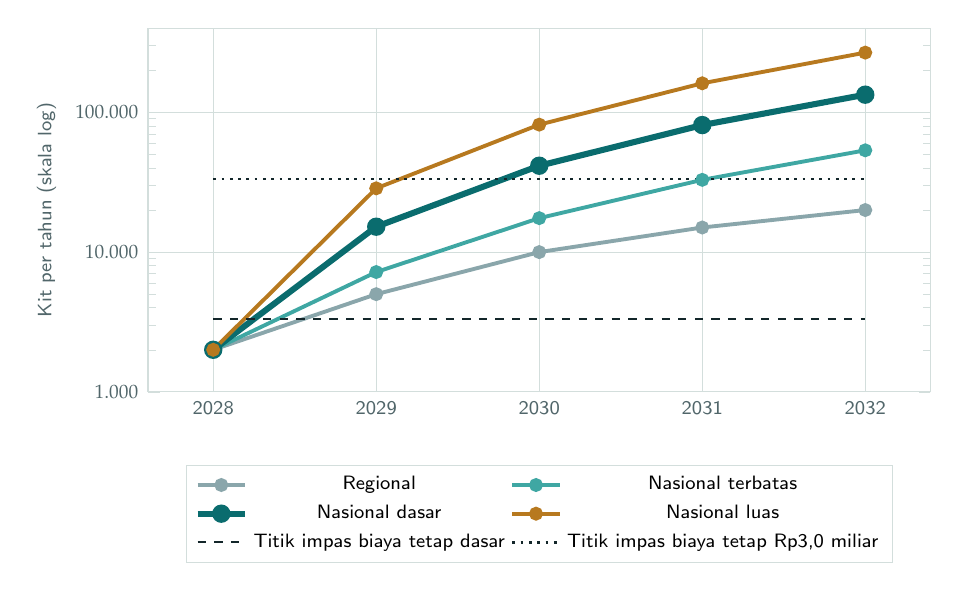
\begin{tikzpicture}
\begin{axis}[natplot,ymode=log,log ticks with fixed point,ymin=1000,ymax=400000,ylabel={Kit per tahun (skala log)},
  legend columns=2]
\addplot[color=sr1,line width=1.4pt,mark=*,mark size=1.8pt] coordinates {(1,2000) (2,5000) (3,10000) (4,15000) (5,20000)};
\addplot[color=sr2,line width=1.4pt,mark=*,mark size=1.8pt] coordinates {(1,2000) (2,7200) (3,17500) (4,32900) (5,53500)};
\addplot[color=sr3,line width=2.2pt,mark=*,mark size=2.2pt] coordinates {(1,2000) (2,15200) (3,41500) (4,81100) (5,133800)};
\addplot[color=sr4,line width=1.4pt,mark=*,mark size=1.8pt] coordinates {(1,2000) (2,28600) (3,81700) (4,161400) (5,267600)};
\addplot[color=ink,dashed,line width=0.8pt,domain=1:5,samples=2] {3334};
\addplot[color=ink,dotted,line width=1pt,domain=1:5,samples=2] {33334};
\legend{Regional,Nasional terbatas,Nasional dasar,Nasional luas,{Titik impas biaya tetap dasar},{Titik impas biaya tetap Rp3,0 miliar}}
\end{axis}
\end{tikzpicture}
\caption{Kit terjual per tahun menurut skenario, dengan titik impas pada dua taraf biaya tetap.}
\label{fig:kits}
\end{figure}

Pada skenario nasional dasar, tahun ke-5 mencapai 133.800 kit, setara 47\% dari skenario konservatif total pasar (0,10\% penduduk per tahun). Skenario nasional luas mencapai 94\% dari angka yang sama, sehingga hanya masuk akal bila pemeriksaan menjadi bagian dari layanan rutin dan produk tidak bersaing dengan produk lain di pasar yang sama.

\subsection{Omzet}

\begin{table}[htbp]
\centering
\caption{Omzet menurut skenario pada harga neto Rp150.000.}
\label{tab:omzet}
\tabstart
\begin{tabular}{@{}lrrrr@{}}
\toprule
\hdrrow\tH{Skenario} & \tH{2028} & \tH{2030} & \tH{2032} & \tH{Total lima tahun} \\
\midrule
Regional & Rp0,30 miliar & Rp1,50 miliar & Rp3,00 miliar & Rp7,80 miliar \\
Nasional terbatas & Rp0,30 miliar & Rp2,62 miliar & Rp8,03 miliar & Rp16,96 miliar \\
Nasional dasar & Rp0,30 miliar & Rp6,22 miliar & Rp20,07 miliar & Rp41,04 miliar \\
Nasional luas & Rp0,30 miliar & Rp12,26 miliar & Rp40,14 miliar & Rp81,19 miliar \\
\bottomrule
\end{tabular}
\end{table}

\subsection{Titik impas}

Titik impas operasional adalah biaya tetap dibagi margin kontribusi. Pada biaya tetap dasar, Rp300 juta $\div$ Rp90.000 = 3.333,3, dibulatkan menjadi 3.334 kit per tahun. Tabel~\ref{tab:bepn} menunjukkan bagaimana titik impas naik bila biaya tetap skala nasional lebih besar. Meski demikian, titik impas tetap kecil dibanding jumlah fasilitas: bahkan pada biaya tetap 20 kali lipat, dibutuhkan 2,49\% dari seluruh fasilitas mitra BPJS.

\begin{table}[htbp]
\centering
\caption{Titik impas menurut biaya tetap tahunan.}
\label{tab:bepn}
\tabstart
\begin{tabular}{@{}rrrr@{}}
\toprule
\hdrrow\tH{Biaya tetap per tahun} & \tH{Kit per tahun} & \tH{Fasilitas (100 kit)} & \tH{Dari 26.759 fasilitas} \\
\midrule
Rp300 juta & 3.334 & 34 & 0,13\% \\
Rp1.500 juta & 16.667 & 167 & 0,62\% \\
Rp3.000 juta & 33.334 & 334 & 1,25\% \\
Rp6.000 juta & 66.667 & 667 & 2,49\% \\
\bottomrule
\end{tabular}
\end{table}

\subsection{Hasil operasi tahun ke-5 menurut biaya tetap}

Biaya tetap dasar Rp300 juta berlaku untuk skala awal. Distribusi nasional, tim penjualan, pengendalian mutu, dukungan lapangan, dan pemantauan keamanan hampir pasti menaikkannya. Karena angkanya belum ada, Tabel~\ref{tab:fcsens} menyajikan hasil operasi tahun ke-5 pada beberapa taraf biaya tetap. Pada skenario nasional dasar, kontribusi tahun ke-5 sebesar Rp12,04 miliar menutup biaya tetap sampai kira-kira Rp12,0 miliar per tahun.

\begin{table}[htbp]
\centering
\caption{Hasil operasi tahun ke-5 (sebelum pajak dan investasi awal) menurut biaya tetap.}
\label{tab:fcsens}
\tabstart
\begin{tabular}{@{}lrrrr@{}}
\toprule
\hdrrow\tH{Skenario} & \tH{Rp300 juta (1x)} & \tH{Rp1.500 juta (5x)} & \tH{Rp3.000 juta (10x)} & \tH{Rp6.000 juta (20x)} \\
\midrule
Regional & Rp1.500 juta & Rp300 juta & $-$Rp1.200 juta & $-$Rp4.200 juta \\
Nasional terbatas & Rp4.515 juta & Rp3.315 juta & Rp1.815 juta & $-$Rp1.185 juta \\
Nasional dasar & Rp11.742 juta & Rp10.542 juta & Rp9.042 juta & Rp6.042 juta \\
Nasional luas & Rp23.784 juta & Rp22.584 juta & Rp21.084 juta & Rp18.084 juta \\
\bottomrule
\end{tabular}
\end{table}

\begin{catatan}[Temuan]
Skenario regional hanya layak bila biaya tetap tetap kecil. Pada biaya tetap lima kali lipat hasilnya turun menjadi Rp300 juta, dan pada sepuluh kali lipat menjadi negatif. Skala nasional memberi ruang bagi struktur biaya yang profesional, tetapi hanya bila adopsi benar-benar tercapai.
\end{catatan}

\subsection{Investasi maksimum dan payback}

Karena investasi awal belum tersedia, Tabel~\ref{tab:maxinv} membalik pertanyaan: berapa investasi (validasi klinis, registrasi, fasilitas produksi) yang masih menghasilkan NPV nol, dengan investasi dikeluarkan pertengahan 2027 (0,7 tahun dari tanggal dokumen), arus operasi 2028 sampai 2032, diskonto 20\%, tanpa pajak dan nilai akhir. Tabel~\ref{tab:pbn} memberi payback pada biaya tetap acuan Rp3,0 miliar per tahun.

\begin{table}[htbp]
\centering
\caption{Investasi awal maksimum untuk NPV nol (diskonto 20\%) menurut skenario dan biaya tetap.}
\label{tab:maxinv}
\tabstart
\begin{tabular}{@{}lrrrr@{}}
\toprule
\hdrrow\tH{Skenario} & \tH{Biaya tetap 1x} & \tH{5x} & \tH{10x} & \tH{20x} \\
\midrule
Regional & Rp1,5 miliar & tidak ada & tidak ada & tidak ada \\
Nasional terbatas & Rp4,0 miliar & Rp0,4 miliar & tidak ada & tidak ada \\
Nasional dasar & Rp10,7 miliar & Rp7,1 miliar & Rp2,6 miliar & tidak ada \\
Nasional luas & Rp22,0 miliar & Rp18,4 miliar & Rp13,9 miliar & Rp4,9 miliar \\
\bottomrule
\end{tabular}
\end{table}

\begin{table}[htbp]
\centering
\caption{Payback (tahun sejak awal penjualan) pada biaya tetap Rp3,0 miliar per tahun.}
\label{tab:pbn}
\tabstart
\begin{tabular}{@{}lrrrr@{}}
\toprule
\hdrrow\tH{Investasi awal} & \tH{Regional} & \tH{Nasional terbatas} & \tH{Nasional dasar} & \tH{Nasional luas} \\
\midrule
Rp1 miliar & lebih dari 5 tahun & lebih dari 5 tahun & 4,0 tahun & 3,0 tahun \\
Rp3 miliar & lebih dari 5 tahun & lebih dari 5 tahun & 4,3 tahun & 3,2 tahun \\
Rp5 miliar & lebih dari 5 tahun & lebih dari 5 tahun & 4,5 tahun & 3,3 tahun \\
Rp10 miliar & lebih dari 5 tahun & lebih dari 5 tahun & lebih dari 5 tahun & 3,8 tahun \\
\bottomrule
\end{tabular}
\end{table}

Pembacaannya: bila validasi klinis, registrasi, dan fasilitas produksi total berbiaya sekitar Rp3 miliar, hanya skenario nasional dasar dan luas yang kembali modal dalam lima tahun pada biaya tetap acuan. Angka investasi harus diisi tim sebelum studi ini dipakai sebagai dasar keputusan.

\subsection{Sensitivitas}

Tabel~\ref{tab:tor} menguji hasil operasi tahun ke-5 skenario nasional dasar pada biaya tetap acuan (dasar Rp9.042 juta) terhadap perubahan satu parameter. Harga dan volume paling berpengaruh. Hasilnya tetap positif pada semua sisi buruk.

\begin{table}[htbp]
\centering
\caption{Hasil operasi tahun ke-5, skenario nasional dasar, bila satu parameter berubah.}
\label{tab:tor}
\tabstart
\begin{tabular}{@{}lrr@{}}
\toprule
\hdrrow\tH{Parameter yang diubah} & \tH{Sisi buruk} & \tH{Sisi baik} \\
\midrule
Volume (30\%) & Rp5.429 juta & Rp12.655 juta \\
Harga neto (20\%) & Rp5.028 juta & Rp13.056 juta \\
Biaya variabel (25\%) & Rp7.035 juta & Rp11.049 juta \\
Biaya tetap (50\%) & Rp7.542 juta & Rp10.542 juta \\
\bottomrule
\end{tabular}
\end{table}

Tabel~\ref{tab:bep} menunjukkan titik impas (kit per tahun) pada kombinasi harga neto dan biaya variabel dengan biaya tetap Rp300 juta.

\begin{table}[htbp]
\centering
\caption{Titik impas (kit per tahun) menurut harga neto (kolom) dan biaya variabel (baris).}
\label{tab:bep}
\tabstart
\begin{tabular}{@{}lrrrrr@{}}
\toprule
\hdrrow\tH{Biaya variabel} & \tH{Rp120.000} & \tH{Rp135.000} & \tH{Rp150.000} & \tH{Rp165.000} & \tH{Rp180.000} \\
\midrule
Rp45.000 & 4.000 & 3.334 & 2.858 & 2.500 & 2.223 \\
Rp60.000 & 5.000 & 4.000 & 3.334 & 2.858 & 2.500 \\
Rp75.000 & 6.667 & 5.000 & 4.000 & 3.334 & 2.858 \\
Rp90.000 & 10.000 & 6.667 & 5.000 & 4.000 & 3.334 \\
\bottomrule
\end{tabular}
\end{table}

\section{Kapasitas produksi dan rantai pasok}

Skala nasional mengubah pertanyaan dari apakah ada permintaan menjadi apakah produksi dapat mengikutinya. Tabel~\ref{tab:cap} menerjemahkan volume tahun ke-5 menjadi beban produksi. Pada skenario nasional dasar, produksi sekitar 11.150 kit per bulan atau 535 kit per hari kerja (250 hari), dengan sekitar 1,34 juta sumur terisi ekstrak setiap tahun.

\begin{table}[htbp]
\centering
\caption{Kebutuhan produksi tahun ke-5 (250 hari kerja; 10 sumur per kit).}
\label{tab:cap}
\tabstart
\begin{tabular}{@{}lrrrr@{}}
\toprule
\hdrrow\tH{Skenario} & \tH{Kit per tahun} & \tH{Kit per bulan} & \tH{Kit per hari kerja} & \tH{Sumur per tahun} \\
\midrule
Regional & 20.000 & 1.667 & 80 & 0,20 juta \\
Nasional terbatas & 53.500 & 4.458 & 214 & 0,54 juta \\
Nasional dasar & 133.800 & 11.150 & 535 & 1,34 juta \\
Nasional luas & 267.600 & 22.300 & 1.070 & 2,68 juta \\
\bottomrule
\end{tabular}
\end{table}

Beberapa hal belum diketahui dan menentukan kelayakan pada skala ini: kapasitas per batch, umur simpan dan kondisi penyimpanan kit (rantai dingin atau tidak), pasokan bahan baku ekstrak alergen yang terstandar, dan waktu rilis per batch. Pedoman Badan Obat Eropa untuk produk alergen menekankan standardisasi bahan awal dan konsistensi antar batch \cite{ema}. Untuk distribusi antarpulau, umur simpan dan kondisi penyimpanan menentukan apakah pengiriman ke Indonesia timur dapat dilakukan lewat distributor biasa. Dua hal ini dijawab oleh data Certificate of Analysis dan uji stabilitas yang tercantum pada dokumen CoA dan dokumen teknis produksi.

\section{Kekayaan intelektual dan ilustrasi valuasi}

Paten Sederhana IDS000011522 diterima 11 Agustus 2022 dan diberikan 14 Oktober 2025 (permohonan S00202208501). Paten sederhana berlaku 10 tahun sejak tanggal penerimaan dan tidak dapat diperpanjang (UU Nomor 13 Tahun 2016 tentang Paten, Pasal 22, dikutip melalui \cite{izin}), sehingga perlindungan berakhir 11 Agustus 2032. Bila penjualan dimulai 1 Januari 2028, produk terlindungi paten selama 4,6 tahun, dan tahun ke-5 hanya terlindungi selama 7,3 bulan.

Tabel~\ref{tab:ip} adalah ilustrasi metode relief from royalty: nilai kini royalti atas penjualan lisensiat selama masa paten, pada diskonto 20\%. Tarif royalti yang diuji bersumber dari tolok ukur terbuka: median lintas tahap 2,38\% pada lisensi universitas ke perusahaan rintisan di ilmu hayati \cite{gd}, median sekitar 3\% dari penjualan neto pada lisensi delapan universitas Amerika \cite{bvr}, dan 65\% dari seluruh tarif royalti lintas industri berada pada 5\% atau kurang \cite{lesi}. Tolok ukur ini bukan khusus diagnostik, sehingga hanya memberi rentang kasar.

\begin{table}[htbp]
\centering
\caption{Nilai kini royalti selama masa paten (diskonto 20\%).}
\label{tab:ip}
\tabstart
\begin{tabular}{@{}lrrrr@{}}
\toprule
\hdrrow\tH{Skenario} & \tH{Penjualan neto} & \tH{Royalti 2,4\%} & \tH{Royalti 3\%} & \tH{Royalti 5\%} \\
\midrule
Regional & Rp6,63 miliar & Rp74 juta & Rp92 juta & Rp154 juta \\
Nasional terbatas & Rp13,83 miliar & Rp147 juta & Rp184 juta & Rp306 juta \\
Nasional dasar & Rp33,20 miliar & Rp347 juta & Rp434 juta & Rp724 juta \\
Nasional luas & Rp65,51 miliar & Rp682 juta & Rp853 juta & Rp1.421 juta \\
\bottomrule
\end{tabular}
\end{table}

Pada skenario nasional dasar, penjualan neto selama masa paten Rp33,20 miliar dan nilai kini royalti berkisar Rp290 juta sampai Rp876 juta untuk diskonto 15\% sampai 25\%. Pada skenario regional rentangnya Rp63 juta sampai Rp183 juta, dan pada skenario nasional luas paling tinggi Rp1.723 juta. Ilustrasi ini bukan laporan penilaian oleh penilai profesional. Bahkan pada skala nasional, royalti satu paten sederhana dengan sisa masa kurang dari enam tahun bernilai di bawah Rp2 miliar. Nilai komersial yang lebih besar bertumpu pada tiga hal berikut.

\begin{enumerate}
\item Volume dan perluasan portofolio (lebih banyak alergen dan lini produk lain di luar patch).
\item Pengetahuan teknis yang tidak ikut gugur bersama paten: formulasi pembawa, metode standardisasi ekstrak, dan prosedur mutu.
\item Lapisan perlindungan tambahan: paten untuk penyempurnaan, hak cipta untuk aplikasi pembaca, dan desain industri untuk kemasan.
\end{enumerate}

Biaya lisensi di muka dan pembayaran tahap (milestone) tidak dimodelkan. Pada survei lisensi universitas ilmu hayati, 75\% perjanjian memuat biaya di muka dengan median USD 17.500 \cite{gd}, sehingga komponen ini kecil bila tidak dinegosiasikan khusus.

\section{Regulasi dan jalur izin edar}

Produk alergen untuk diagnosis in vivo umumnya diatur sebagai produk obat atau biologik. Pedoman European Medicines Agency mencakup ekstrak alergen dan alergen rekombinan untuk imunoterapi spesifik maupun diagnosis in vivo penyakit alergi yang dimediasi IgE \cite{ema}, dan T.R.U.E. TEST dilisensikan sebagai biologik di Amerika Serikat \cite{fda}.

Di Indonesia, registrasi obat mengikuti Peraturan BPOM Nomor 24 Tahun 2017 beserta perubahannya, terakhir Peraturan BPOM Nomor 15 Tahun 2023 \cite{hukumonline}. Menurut ringkasan Peraturan Pemerintah Nomor 15 Tahun 2026 tentang penerimaan negara bukan pajak BPOM, tarif registrasi produk biologi baru adalah Rp30 juta dan evaluasi persetujuan uji klinik Rp5 juta, dengan tarif Rp0 untuk jasa registrasi produsen mikro dan kecil dalam negeri; cakupan pembebasan itu tidak dirinci pada ringkasan tersebut \cite{pp15}. Klasifikasi akhir produk ini (produk biologi atau alat kesehatan) belum dikonfirmasi. Konsultasi pra-registrasi dengan BPOM dianjurkan sebelum biaya validasi dikeluarkan. Biaya registrasi relatif kecil dibanding biaya validasi klinis, kepatuhan cara pembuatan yang baik, dan studi stabilitas, yang menjadi komponen utama investasi awal.

Untuk peluncuran nasional, izin edar berlaku di seluruh wilayah, tetapi persyaratan penyalur dan penyimpanan di tiap provinsi perlu dipetakan oleh mitra distribusi sebelum Fase 2.

\section{Risiko dan mitigasi}

\begin{table}[htbp]
\centering
\caption{Risiko utama dan langkah mitigasi.}
\label{tab:risk}
\tabstart
\begin{tabular}{@{}L{4.2cm}L{5.2cm}L{5.5cm}@{}}
\toprule
\hdrrow\tH{Risiko} & \tH{Dasar} & \tH{Mitigasi} \\
\midrule
Klasifikasi dan jalur izin edar belum pasti & Produk biologi dan alat kesehatan memiliki persyaratan berbeda & Konsultasi pra-registrasi BPOM; siapkan berkas untuk kedua jalur \\
Validitas klinis belum terbukti & Landasan baru berupa studi in vitro & Studi validasi terhadap uji tusuk kulit dan IgE spesifik; tetapkan kriteria baca sebelum studi \\
Konsistensi ekstrak antar batch & Ekstrak alergen perlu standardisasi mutu \cite{ema} & CoA per batch dengan spesifikasi tertulis dan uji stabilitas \\
Kapasitas produksi tidak mengikuti adopsi & Skenario nasional dasar butuh sekitar 11.150 kit per bulan & Perjanjian kapasitas dengan mitra produksi; adopsi bertahap per fase \\
Distribusi antarpulau dan umur simpan & Konsentrasi penduduk di Jawa; Indonesia timur 3,17\% penduduk & Uji stabilitas; mitra distributor regional; Fase 4 setelah teruji \\
Biaya tetap skala nasional lebih besar & Biaya tetap dasar hanya untuk skala awal & Anggaran biaya tetap rinci sebelum Fase 2; lihat Tabel~\ref{tab:fcsens} \\
Masa paten pendek & Berakhir 11 Agustus 2032 & Lapisan IP tambahan; percepat awal penjualan \\
Mitra belum mengikat & Kerja sama masih penjajakan & Surat minat atau nota kesepahaman dengan syarat lisensi dan target volume \\
Adopsi, harga, dan penjaminan & Harga neto bukan harga ke pasien; pembiayaan JKN belum diketahui & Pilot di fasilitas terpilih; pantau tarif akhir; dialog dengan pemangku kebijakan \\
\bottomrule
\end{tabular}
\end{table}

\section{Data yang akan melengkapi studi}

Beberapa input belum tersedia dan menentukan hasil akhir: investasi awal dan anggaran uji klinis, biaya fasilitas produksi dan cara pembuatan yang baik, rincian biaya tetap pada skala nasional, struktur lisensi dengan mitra produksi, kapasitas per batch, umur simpan, sebaran fasilitas dan harga tes alergi per provinsi (panel kecil, uji tusuk kulit, dan IgE satuan, lengkap dengan jumlah alergen), dan skema penjaminan. Setelah data ini tersedia, skrip model dijalankan ulang dan Tabel~\ref{tab:faskes} sampai \ref{tab:ip} diperbarui.

\begin{thebibliography}{99}\small\raggedright
\setlength{\itemsep}{2pt}
\bibitem{gmi} Global Market Insights. Allergy Diagnostics Market. Diakses Oktober 2026. \url{https://www.gminsights.com/industry-analysis/allergy-diagnostics-market}
\bibitem{rm} ResearchAndMarkets.com. Global Allergy Diagnostics Market Report 2025. GlobeNewswire, 1 Mei 2025. \url{https://www.globenewswire.com/news-release/2025/05/01/3072134/28124/en/Global-Allergy-Diagnostics-Market-Report-2025-Forecast-to-Reach-13-4-Billion-by-2034-Reimbursement-Support-and-Technological-Innovation-Drive-Growth-at-a-CAGR-of-9-20.html}
\bibitem{bps} BPS. Hasil Survei Penduduk Antar Sensus (SUPAS) 2025: 284,67 juta jiwa. Dikutip melalui Bisnis.com, 5 Mei 2026. \url{https://kabar24.bisnis.com/read/20260505/15/1971460/sensus-bps-jumlah-penduduk-ri-capai-28467-juta-jiwa-2025-tumbuh-melambat}
\bibitem{sensus} Sekretariat Kabinet RI. Hasil Sensus Penduduk 2020; BPS: Meski lambat, ada pergeseran penduduk antarpulau. \url{https://setkab.go.id/hasil-sensus-penduduk-2020-bps-meski-lambat-ada-pergeseran-penduduk-antarpulau/}
\bibitem{bpjs} Bisnis.com. BPJS Kesehatan klaim kerja sama dengan 3.120 RS pada 2023. 14 Januari 2024. \url{https://finansial.bisnis.com/read/20240114/215/1732195/bpjs-kesehatan-klaim-kerja-sama-dengan-3120-rs-pada-2023}
\bibitem{jkn} Warta Ekonomi. Cakupan JKN tembus 98 persen penduduk Indonesia, BPJS catat peserta capai 282,7 juta jiwa. 27 Januari 2026. \url{https://wartaekonomi.co.id/read598290/cakupan-jkn-tembus-98-penduduk-indonesia-bpjs-catat-peserta-capai-2827-juta-jiwa}
\bibitem{alodokter} Alodokter. Tes Alergi, daftar tarif fasilitas di Surabaya. Diakses Oktober 2026. \url{https://www.alodokter.com/cari-rumah-sakit/kulit-dan-kelamin/tes-alergi/surabaya}
\bibitem{royal} Rumah Sakit Royal Progress. Paket Cek Alergi, IgE Atopy 54 Alergen (Rp2.200.000, termasuk konsultasi dokter). Diakses Oktober 2026. \url{https://oncare.royalprogress.com/en/s/rumah-sakit-royal-progress/detail-produk/paket-cek-alergi-ige-54-alergen}
\bibitem{medicastore} Medicastore. Tes Alergi (uji tusuk kulit 33 alergen Rp350.000 sampai Rp600.000; IgE spesifik Rp200.000 sampai Rp300.000 per alergen). 9 Januari 2009. \url{https://medicastore.com/artikel/1964/tes-alergi}
\bibitem{pramita} Laboratorium Klinik Pramita. Allergy Test Panels (IgE spesifik 96 alergen; harga tidak dicantumkan). 2 Oktober 2025. \url{https://pramita.co.id/en/inspiration/allergy-test-panels}
\bibitem{pramita2} Laboratorium Klinik Pramita. Food Allergy Check Panel (IgE spesifik 54 jenis; IgG Food Tolerance 46 jenis makanan; harga tidak dicantumkan). Diakses Oktober 2026. \url{https://pramita.co.id/en/inspiration/food-allergy-check-panel}
\bibitem{tim} Daftar harga tes alergi pada Siloam Hospitals, Tirta Medical Centre, RS Mitra Keluarga, Klinik Utama DR Indrajana, dan Laboratorium Klinik Pramita. Dihimpun Oktober 2026.
\bibitem{fda} FDA, Center for Biologics Evaluation and Research. Safety and utilization review for the Pediatric Advisory Committee (T.R.U.E. TEST, STN 103738), September 2021. \url{https://www.fda.gov/media/151565/download}
\bibitem{ema} European Medicines Agency. Allergen products: production and quality issues, EMEA/CHMP/BWP/304831/2007, berlaku 20 Mei 2009. \url{https://www.ema.europa.eu/en/allergen-products-production-quality-issues-scientific-guideline}
\bibitem{biofarma} Bio Farma. Bio Farma segera luncurkan pendeteksi diabetes mellitus tipe I. Pengumuman Bio Farma. \url{https://www.biofarma.co.id/en/announcement/detail/bio-farma-segera-luncurkan-pendeteksi-diabetes-mellitus-type-i}
\bibitem{ekatalog} Kabarbursa.com. Pemerintah genjot produk lokal masuk e-katalog LKPP. 16 Oktober 2025. \url{https://www.kabarbursa.com/makro/pemerintah-genjot-produk-lokal-masuk-e-katalog-lkpp}
\bibitem{p3dn} BCA Sekuritas. Kemenperin perkuat pasar industri alat kesehatan lewat P3DN. 8 September 2025. \url{https://bcasekuritas.co.id/latest-news/news/kemenperin-perkuat-pasar-industri-alat-kesehatan-lewat-p3dn}
\bibitem{kemkes88} Kementerian Kesehatan RI. Pemerintah targetkan 60 persen produksi alkes gunakan komponen lokal. 27 Agustus 2022. \url{https://www.kemkes.go.id/id/pemerintah-targetkan-60-persen-produksi-alkes-gunakan-komponen-lokal}
\bibitem{cermati} Cermati Invest. Weekly Update 19 Oktober 2026. \url{https://invest.cermati.com/artikel/amp/cermati-invest-weekly-update-19-oktober-2026}
\bibitem{izin} Izin.co.id. Jangka waktu paten di Indonesia. Diakses Oktober 2026. \url{https://izin.co.id/blog/jangka-waktu-paten/}
\bibitem{gd} Gunderson Dettmer. University License Presentation, 7 Februari 2024. \url{https://www.gunder.com/content/uploads/2024/02/Gunderson-Dettmer-University-License-Presentation-2-7-24.pdf}
\bibitem{bvr} BVWire. Royalty rates for university-bred technology. Isu 186-3, 21 Maret 2018. \url{https://www.bvresources.com/articles/bvwire/royalty-rates-for-university-bred-technology}
\bibitem{lesi} Licensing Executives Society International. Royalty rates and license fees for technology. \url{https://lesi.org/wp-content/uploads/2024/04/royalty-rates-license-fees-for-technology.pdf}
\bibitem{hukumonline} Hukumonline Pro. Drug registration procedures updated: BPOM releases list of 11 biological products and expands evaluation pathways. 19 Agustus 2025 (ringkasan terbuka). \url{https://pro.hukumonline.com/a/lt68a3dbcf7be8e/drug-registration-procedures-updated--bpom-releases-list-of-11-biological-products-and-expands-evaluation-pathways/}
\bibitem{pp15} Veritask. Peraturan Pemerintah Nomor 15 Tahun 2026 mengubah struktur tarif registrasi, inspeksi, dan sertifikasi pada BPOM. Diakses Oktober 2026. \url{https://veritask.ai/id/artikel/peraturan-pemerintah-nomor-15-tahun-2026-mengubah-struktur-tarif-registrasi-inspeksi-dan-sertifikasi-pada-badan-pengawas-obat-dan-makanan}
\end{thebibliography}

\end{document}
